%\documentclass[en,hazy,blue,screen,14pt]{elegantnote}
\documentclass[en,hazy,blue]{elegantnote}
\usepackage[T1]{fontenc}
\usepackage[latin9]{inputenc}
% \usepackage[USenglish]{babel}
\usepackage{babel}
\usepackage{float}
\usepackage{textcomp}
\usepackage{amsmath,amsfonts,amssymb}
\usepackage{amsthm}
\usepackage{graphicx}
\usepackage[ruled,vlined]{algorithm2e}
\PassOptionsToPackage{normalem}{ulem}
\usepackage{ulem}
\usepackage{mathtools}
\usepackage{url}
\usepackage{hyperref}
\usepackage{listings}

%%%%%%%%%%%%%%%%%%%%%%%%%%%%%%%%%%%%%%%
% Math Symbols
%%%%%%%%%%%%%%%%%%%%%%%%%%%%%%%%%%%%%%%
\renewcommand{\>}{{\rightarrow}}
\renewcommand{\hat}{\widehat}
\renewcommand{\tilde}{\widetilde}
\newcommand{\half}{\frac{1}{2}}
%
\newcommand{\R}{{\mathbb R}}
\newcommand{\Z}{{\mathbb Z}}
\newcommand{\N}{{\mathbb N}}
\renewcommand{\P}{{\mathbf P}}
\newcommand{\E}{{\mathbf E}}
\newcommand{\Var}{{\mathbf{Var}}}
\newcommand{\I}{{\mathbf I}}
\newcommand{\1}{{\mathbf 1}}
\newcommand{\0}{{\mathbf 0}}
%%%%%%%%%%%%%%%%%%%%%%%%%%%%%%%%%%%%%%%
% Code Style
%%%%%%%%%%%%%%%%%%%%%%%%%%%%%%%%%%%%%%%
\lstset{
	numbers=left, 
	numberstyle=\small, 
	numbersep=8pt, 
	frame = single, 
	framexleftmargin=15pt,
	breaklines=true,
	columns=fullflexible
}
%%%%%%%%%%%%%%%%%%%%%%%%%%%%%%%%%%%%%%%
% Theorem
%%%%%%%%%%%%%%%%%%%%%%%%%%%%%%%%%%%%%%%
\renewcommand\qedsymbol{$\blacksquare$}
\DeclarePairedDelimiter{\ceil}{\lceil}{\rceil}
\newcommand\tab[1][1cm]{\hspace*{#1}}
\newenvironment{claim}[1]{\par\noindent\underline{Claim:}\space#1}{}
\newenvironment{claimproof}[1]{\par\noindent\underline{Proof:}\space#1}{\hfill $\blacksquare$}

%%%%%%%%%%%%%%%%%%%%%%%%%%%%%%%%%%%%%%%
% Title
%%%%%%%%%%%%%%%%%%%%%%%%%%%%%%%%%%%%%%%
\title{Class Notes: STAT 501\\ Nonparametrics \& Log-Linear Models\\ Ansari-Bradley Test, Kruskal-Wallis Test
}
\author{Da Kuang}
\institute{University of Pennsylvania}
% \version{1.00}
\date{}

\begin{document}

\maketitle
\newpage
\tableofcontents

\newpage
\section{Ansari-Bradley Test}
\subsection{Background}
\subsubsection{$\chi^2$ Distribution and $F$ Distribution}
The $\chi^2$ distribution is obtained directly from independent, standard normal random variables. Let $Z_i$, $i = 1,2, \dots, n$, be $n$ independent random variables, each distribution as standard normal. Define a new random variable as the sum of the squares of the $Z_i$:
\[X = \sum_{i=1}^{n}Z_i^2\]
Then, $X$ has what is known as a $\chi^2$ distribution with $n$ degree of freedom.

Another important distribution for statistics and econometrics is the $F$ distribution. In particular, the $F$ distribution will be used for testing hypotheses in the context of multiple regression analysis.

To define an $F$ random variable, Let $X_1 ~ \chi_{k_1}^2$ and $X_2 ~ \chi_{k_2}^2$ and assume that $X_1$ and $X_2$ are independent. Then the random variable
\[F = \frac{X_1 / k_1}{X_2 / k_2}\]
has an $F$ distribution with $(k_1, k_2)$ degree of freedom. We denote this as $F ~ F_{k_1, k_2}$.
\subsubsection{$F$-test of Equality of Variances}
In statistics, an $F$-test of equality of variances is a test for the null hypothesis that two normal populations have the same variance. 

\begin{itemize}
	\item Let $X_1, \dots, X_n$ and $Y_i, \dots, Y_n$ be iid samples from two populations which each has a normal distribution.
	\item The expected values for the two populations can be different.
	\item The Hypothesis is that the variances are equal.
\end{itemize}

Sample means are 
\[\bar{X} = \frac{1}{n} \sum_{i = 1}^{n} X_i, ~\bar{Y} = \frac{1}{m} \sum_{i=1}^{m}.\]

Sample variances are
\[S_X^2 = \frac{1}{n-1} \sum_{i=1}^{n}(X_i - \bar{X})^2, ~S_Y^2 = \frac{1}{m-1} \sum_{i=1}^{m}(Y_i - \bar{Y})^2.\]

Then the test statistic is an $F$-distribution with $n-1$ and $m-1$ degrees of freedom if the null hypothesis of equality of variacne is true.
\[F = \frac{S_X^2}{S_Y^2}\]

Otherwise it follows an $F$-distribution scaled by the ratio of true variances. The null hypothesis is rejected if $F$ is either too large or too small based on the desired alpha level 


\subsection{Assumption}
Ansari-Bradley Test is an non-parametric version of $F$-test. The null hypothesis of interest here is that the $X$ and $Y$ variable have the same probability distribution but their common distribution is not specified. 

We have the following assumptions for Ansari-Bradley Test:
\begin{itemize}
	\item $X_i$, $i \le m$, iid from continues population 1 with distribution $F$;
	\item $Y_j$, $j \le n$, iid from continues population 2 with distribution $G$;
	\item $X_i's$ and $Y_j's$ mutually independent;
	\item $F$ and $G$  have the same median $\theta$.
\end{itemize}
Note that $X_i$ and $Y_i$ are continues random variable. Also, Ansari-Bradley test works with different median between samples but here we assume two samples have the same median, $\theta$, for simplicity.

The alternative hypothesis can be that $Y$ population has the same general form as the $X$ population, but they could have different scales. It can be written as 
\[\frac{X - \theta}{\eta_x} \stackrel{d}{=} \frac{Y - \theta}{\eta_y}\]

, where $\stackrel{d}{=}$ means ``has the same distribution'', $\eta_x$ and $\eta_y$ are the scale parameters of $F$ and $G$, respectively.

The parameter of interest is the ratio of the scale parameters, $\gamma = \frac{\eta_x}{\eta_y}$.

In terms of this location-scale parameter model with equal location parameters, the null hypothesis is 
\[H_0: \gamma^2 = 1\]
, corresponding to the assertion that the population scale parameters are equal.

why $\gamma^2$ instead of $\gamma$. Sometimes we cannot calculate the variance (second moment), e.g. Poisson Distribution, during  standardization, so we keep the squaring later after the standardization.
\subsection{Hypothesis Test}

\begin{itemize}
	\item $H_0: \gamma^2 = 1$
	\item $H_1: \gamma^2 > 1$ (right-tailed test)
	\item $H_1: \gamma^2 < 1$ (left-tailed test)
	\item $H_1: \gamma^2 \neq 1$ (two-sided test)
\end{itemize}

\subsubsection{Assign Scores}
Order the combined samples of $N = m + n$ $X_i's$ and $Y_j$'s from least to greatest.
\begin{itemize}
	\item Assign the score 1 to both the smallest and the largest observations in this combined sample.
	\item Assign the score 2 to the 2nd smallest and 2nd largest.
	\item ...
\end{itemize}
In the end, we will get a list of score such that
\begin{itemize}
	\item If $N$ is an even integer, the array of assigned scores is 
	\[1, 2, \dots, \frac{N}{2}, \frac{N}{2}, \dots, 2, 1\]
	\item If $N$ is an odd integer, the array of assigned score is 
	\[1, 2, \dots, \frac{N-1}{2},\frac{N+1}{2},\frac{N-1}{2}, \dots, 2, 1\]
\end{itemize}
\subsubsection{Two-sample Scale Statistic}
Let $R_j$ be the score assigned to $Y_j$, $j = 1, \dots, n$.
The test statistic is $C = \sum_{j=1}^{n} R_j$.

Under the null hypothesis, we have
\[\E C = \frac{n(N+2)}{4}, \Var C = \frac{mn(N+2)}{48(N-1)}\]

The big idea is that we calculate the critical value $c_\alpha$ based on the Type I error of the experiment design and decide whether to reject the null hypothesis by comparing $C$ and $c_\alpha$. Intuitively, \textbf{if $\gamma^2 > 1$}, the $X$ values would tend to be more spread out than the $Y$ values. Thus, the $Y_j's$ would tend to get larger scores than the $X_i's$. \textbf{Then $C$ would tend to be larger}.

Note that $\gamma$ shows in the hypothesis to describe the data but the test statistics is actually $C$, the sum of ranks in $Y$.

The p-value of the hypothesis test can be calculated from the build-in R function \texttt{ansari.test}.

\begin{center}
	\lstinputlisting[language=R, caption=Ansari Example]{code/ansari.R}
\end{center}

\begin{figure}[H]
	\centering
	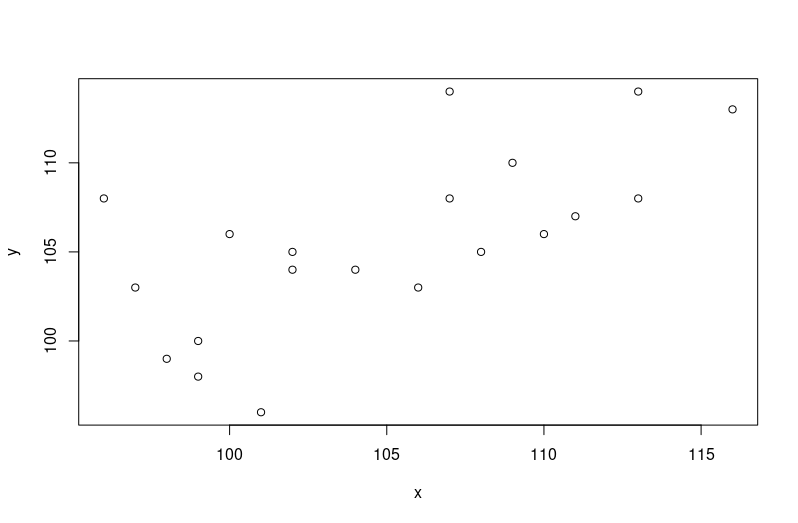
\includegraphics[width=0.7\linewidth]{fig/ansari}
	\caption{}
	\label{fig:ansari}
\end{figure}

Note that the range of X and Y are very similar, which indicates that they share the same dispersion. Also, in the Ansari-Bradley test, we get p-val = 0.1815, so that we cannot reject the null hypothesis.


\section{Kruskal-Wallis Test}
\subsection{Background}
\subsubsection{The One-Way Layout}
One-way, also known as single-factor, means that there is only one treatment among the groups in data. 

Denote the data consist of $N=\sum_{j=1}^{I} n_i$ observations, with $n_i$ observations from the $i$th treatment, $i=1, \dots, I$.

\begin{figure}[H]
	\centering
	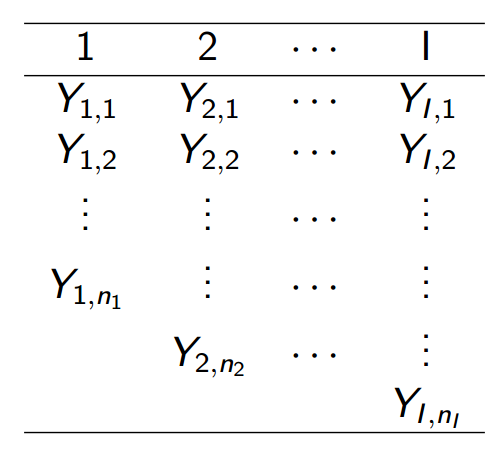
\includegraphics[width=0.3\linewidth]{fig/data}
	\caption{Data}
	\label{fig:data}
\end{figure}

Note that each group can have different number of observations.
\subsubsection{One-Way ANOVA}
In statistics, one-way analysis of variance is a technique that can be used to compare means(location) of two \textbf{or more samples}. The primary interest consist in comparing the location of three of more samples.

\begin{itemize}
	\item Null Hypothesis: the sample data are supposed to come from the same population.
	\item Alternative Hypothesis: the sample data are supposed to come from different populations.
\end{itemize}

Recall in ANOVA, the variability of data is broken down into two components:
\begin{itemize}
	\item Sum of squares of the columns: between groups variability, due to the different locations of the populations.
	\item Sum of squares of the error: within groups variability, due to the variability in the population.
\end{itemize}

\begin{figure}[H]
	\centering
	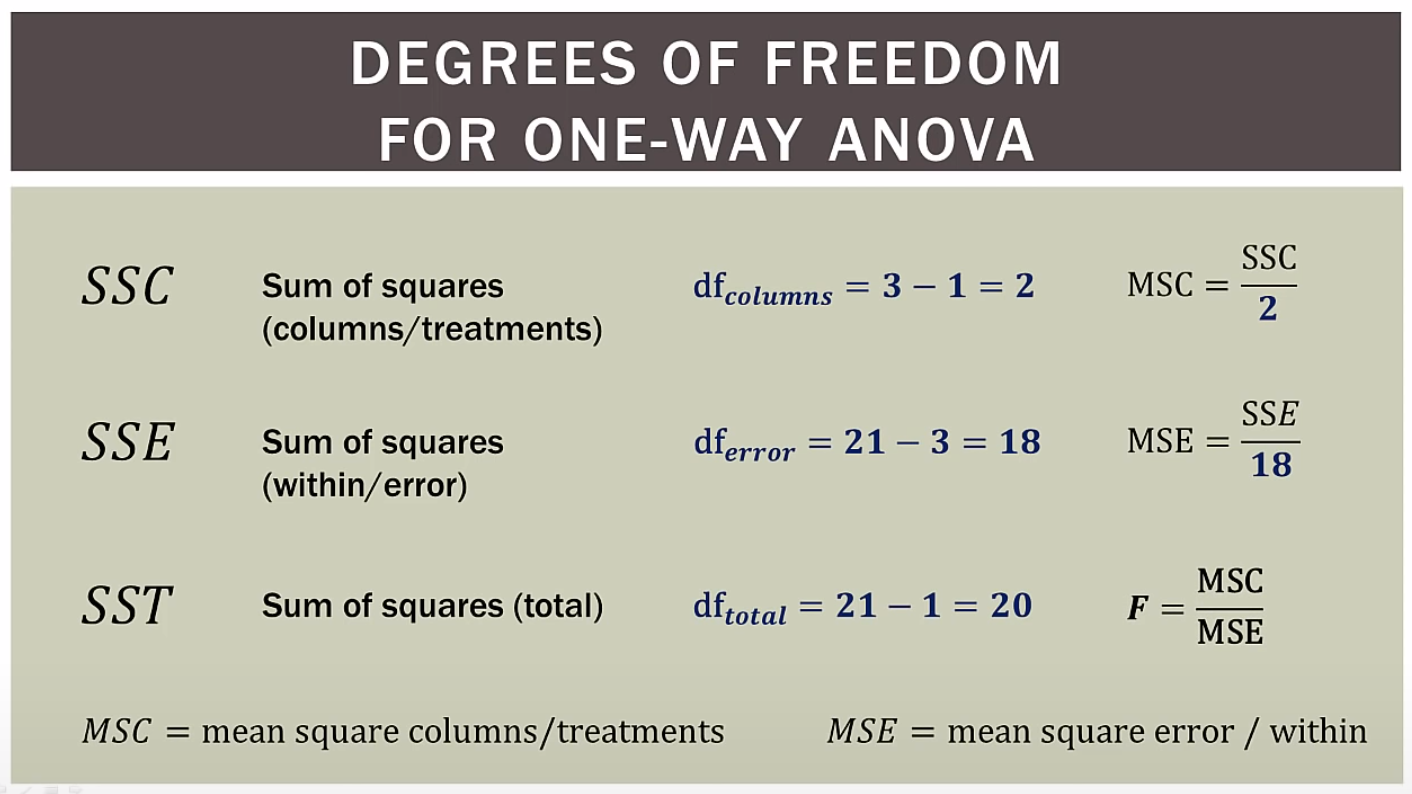
\includegraphics[width=0.7\linewidth]{fig/anova}
	\caption{Analysis of Variance}
	\label{fig:anova}
\end{figure}

$F$-ratio is the test statistic for the hypothesis test.

\subsection{Assumption}
\begin{itemize}
	\item The random variables are all mutually independent.
	\item Random variables in the same group follow the same continuous distribution $F_i$, $i=1, \dots, I$.
	\item $F_i(t) = F(t-\tau_i)$, $-\infty < t < \infty$.
	\begin{itemize}
		\item $F$ is a continuous distribution function with unknown median $\theta$;
		\item $\tau_i$ is the unknown treatment effect for the $i$-th population.
		\item No difference in scale parameters (variability).
	\end{itemize}
\end{itemize}

We can set up the model of each observation based on the assumptions.
\[Y_{ik} = \theta + \tau_i + \epsilon_{ik}\]

\begin{itemize}
	\item $i = 1, \dots, I, k = 1, \dots, n_i$.
	\item $\theta$: overall median.
	\item $\tau_i$: the $i$-th treatment effect.
	\item $\epsilon_{ik}$: random error. iid from a continuous distribution with median 0.
\end{itemize}

\subsection{Hypothesis}
\begin{itemize}
	\item $H_0$: $\tau_1 = \cdots = \tau_I$, which means that $F_1 = \cdots = F_I = F$.
	\item $H_1$: $\tau_1 \dots \tau_I$ are not all equal.
\end{itemize}
\subsubsection{Rank}
Combine all $N$ observations from the $I$ groups and order them from least to greatest.
\begin{figure}[H]
	\centering
	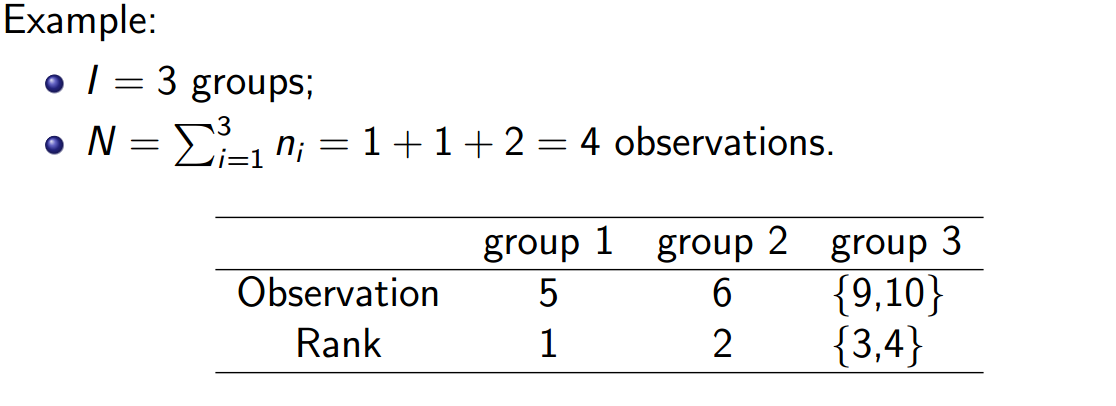
\includegraphics[width=0.7\linewidth]{fig/rank}
	\caption{Example: Rank}
	\label{fig:rank}
\end{figure}

\subsubsection{Test Statistic}

Let $r_{ik}$ denotes the rank of $Y_{ik}$ in this joint ranking. The average rank assigned in the joint ranking is 
\[\frac{1}{N}\sum_{i = 1}^{I} \sum_{k=1}^{n_i} r_{ik} = \frac{N(N+1)}{2N} = \frac{N + 1}{2}\]

Let $R_i = \sum_{k=1}^{n_i} r_{ik}$, which is the sum of the joint ranks received by the observations in the $i$-th group.

Let $\bar{R}_i = R_i / n_i$, $i = 1, \dots, I$, which is the average rank received by observations in the $i$-th group.

The Kruskal-Wallis statistic $H$ is then given by
\begin{align*}
	H 
	&= \frac{12}{N(N+1)} \sum_{i=1}^{I} n_i (\bar{R}_i - \frac{N+1}{2})^2\\
	&= (\frac{12}{N(N+1)} \sum_{i=1}^{I} \frac{R_i^2}{n_i}) - 3(N+1).
\end{align*}

Reject $H_0$ if $H \ge h_\alpha$, the upper $\alpha$ percentile for the null distribution of $H$.

Under the Null Hypothesis, 
\begin{itemize}
	\item $\E r_{ik} = \frac{N+1}{2}$
	\item $\E \bar{R}_i = \frac{1}{n_i} \sum_{k=1}^{n_i} r_{ik} = \frac{1}{n_i} n_i \E r_{ik} = \frac{N + 1}{2}$.
\end{itemize}


Intuitively, we expect the $\bar{R}_i$'s to be close to $\frac{N+1}{2}$ when $H_0$ is true. So that small values of $H$ represent agreement with $H_0$. 

Otherwise, when the $\tau$'s are not all equal, we would expect a portion of the associated treatment average ranks to differ from their common average, $(N+1)/2$, with some tending to be larger and some smaller. Hence, the net result $n_i(\bar{R}_i - \frac{N+1}{2})^2$ would lead to a large value of $H$. This suggests rejecting $H_0$ in favor of $H_1$ for large values of $H$.

\begin{figure}[H]
	\centering
	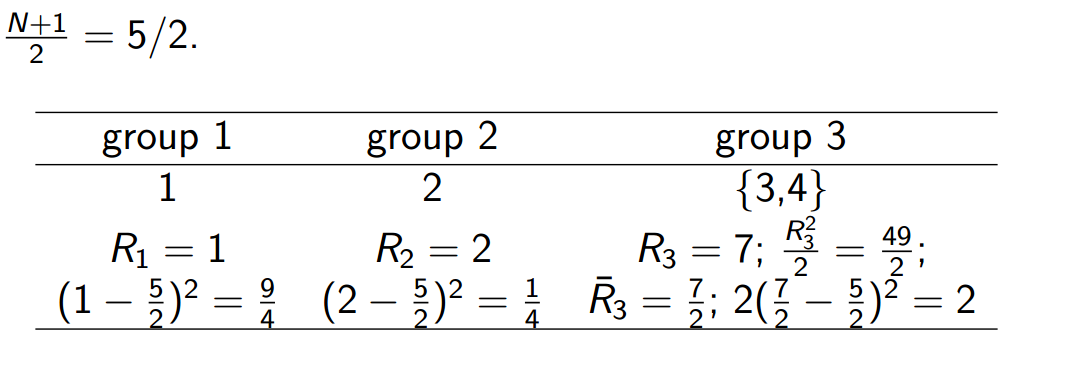
\includegraphics[width=0.7\linewidth]{fig/kruskal-wallis}
	\caption{Example: Kruskal-Wallis Test}
	\label{fig:kruskal-wallis}
\end{figure}

\subsection{Extensions}
Recall that the alternative hypothesis of Kruskal-Wallis Test is that $\tau_i$'s are not equal. Now we introduce two more test for stronger alternative hypothesis.

\subsubsection{Jonckheere-Terpstra Test}
In many practical settings, the treatments are such that the
appropriate alternatives to no differences in treatment effects
(H0) are those of increasing (or decreasing) treatment effects
according to some natural labeling for the treatments.

Examples of such settings include ``treatments'' corresponding to
degrees of knowledge of performance, quality or quantity of
materials, severity of disease, amount of practice, drug dosage
levels, intensity of a stimulus, and temperature.

The Kruskal-Wallis test does not utilize any such partial prior
information regarding a postulated alternative ordering.

The alternative hypothesis for Jonckheere-Terpstra Test is that
\[H_1: \tau_1 \le \tau_2 \le \cdots \le \tau_I\]
, with at least one strict inequality.

\subsubsection{Mack-Wolfe Test}
The alternative hypothesis for Mack-Wolfe Test is that
\[H_1: \tau_1 \le \cdots \le \tau_p \ge \tau_{p+1} \ge \cdots \tau_I\]
, with at least one strict inequality.

The distribution of $\tau_i$'s are in the shape of umbrella. But this test rarely used nowdays.
\end{document}
